\chapter{Circuits}

\paragraph{Objectif}

\begin{enumerate}
  \item L'étudiante comprendra les lois de Kirchhoff et saura les appliquer à
    des circuits composés de piles et de résistances.
  \item L'étudiante saura comment calculer la résistance équivalente à
    des agencements de résistances en série et en parallèle.
\end{enumerate}


\section{Force électromotrice}

\marginnote{
  Tremblay \S 6.1, 6.2

  Lafrance \S 4.9
}

Dans un circuit, il faut quelque chose qui fournit de l'énergie aux charges
pour les mettre en mouvement. Autrement dit, il faut une source de différence
de potentiel. Une source peut être une batterie (qui convertit de l'énergie
chimique en énergie électrique), une centrale hydroélectrique (qui convertit de
l'énergie potentielle gravitationnelle en énergie électrique), une interface
électronique (qui convertit de l'énergie électrique et énergie électrique),
etc. Ces sources font activement un travail pour générer la tension dans le
circuit. On les appelle souvent des sources de \textbf{force électromotrice},
représentée par le symbole \emf.

Attention! Une force électromotrice n'est pas une force, c'est une différence
de potentiel maintenue activement par un processus quelconque dans la source.


\section{Lois de Kirchhoff}

\marginnote{
  Tremblay \S 6.5

  Lafrance \S 7.2
}

\subsection*{Loi des n\oe uds}

Dans notre analyse des circuits, nous supposerons que le courant est constant
ou qu'il varie suffisamment lentement pour que l'équilibre puisse s'établir
dans les fils. Par conséquent, aucune charge ne peut s'accumuler dans les
éléments de circuit (sauf sur les condensateurs).

Si les charges ne peuvent s'accumuler, le courant entrant à chaque point du
circuit doit être le même que le courant sortant de ce point (par conservation
de la charge). C'est la \textbf{loi des n\oe uds}.


\begin{diapobox}
\minisec{Exercice sur la loi des n\oe uds}

Le diagramme ci-dessous illustre un n\oe ud dans un circuit. Les courants sont
\begin{align*}
  I_1 &= \SI{100}{mA} \\
  I_2 &= \SI{45}{mA} \\
  I_3 &= \SI{80}{mA} \\
  I_4 &= \SI{300}{mA} \\
\end{align*}
Déterminer $I_5$ et la direction du courant dans cette branche.

\begin{center}
  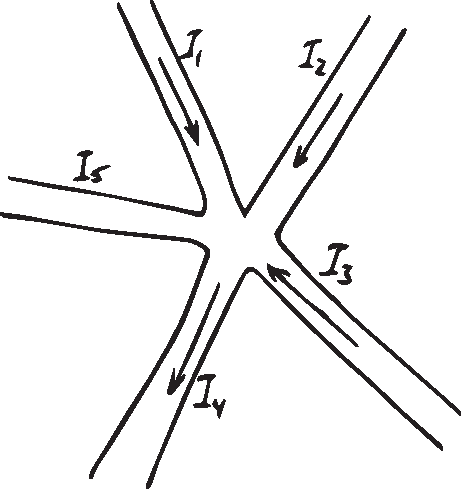
\includegraphics[scale=0.5]{07-circuits-cc/figures/loi-noeuds.pdf}
\end{center}
\end{diapobox}

\begin{reponsebox}
Parmi les courants connus, la somme des courants entrant est
$$I_1 + I_2 + I_3 = \SI{225}{mA}$$
et la somme des courants sortant est
$$I_4 = \SI{300}{mA}.$$
Pour que la loi des noeuds soit satisfait, il faut que
$$I_\mathrm{entrant} = I_\mathrm{sortant}.$$
Par conséquent, le courant $I_5$ doit nécessairement être un courant entrant
d'où
$$I_\mathrm{entrant} = I_1 + I_2 + I_3 + I_5$$
et
$$I_\mathrm{sortant} = I_4.$$
Donc
\begin{align*}
  I_1 + I_2 + I_3 + I_5 &= I_4 \\
  I_5 &= I_4 - I_1 - I_2 - I_3 \\
      &= \SI{75}{mA}
\end{align*}
\end{reponsebox}


\subsection*{Loi des mailles}

Le long de n'importe quel chemin fermé, la somme des différences de potentiel
doit donner $0$. C'est une conséquence du fait que la force électrique est
conservative, autrement dit, c'est parce que l'énergie est conservée.


\begin{diapobox}
\minisec{Exercice sur la loi des mailles}

On considère le circuit suivant dans lequel $\emf = \SI{12}{V}$, $R_1 =
\SI{100}{\ohm}$ et $R_3 = \SI{50}{\ohm}$. Le courant qui circule dans le
circuit est de $I = \SI{30}{mA}$. Déterminer $R_2$.

\begin{center}
  \begin{circuitikz}
    % French babel breaks everything... see https://latex.org/forum/viewtopic.php?t=11981
    \shorthandoff{:}\shorthandoff{!}
    \draw (0, 0) to[battery, l=\emf, invert] (0, 3)
      to[R, l=$R_1$] (4, 3)
      to[R, l=$R_2$] (4, 0);
    \draw (0, 0) to[R, l=$R_3$] (4, 0);
  \end{circuitikz}
\end{center}
\end{diapobox}

\begin{reponsebox}
Si on fait le tour de la maille
$$\emf - R_1 I - R_2 I - R_3 I = 0$$
donc
$$R_2 = \frac{\emf - R_1 I - R_3 I}{I} = \frac{\emf}{I} - R_1 - R_3$$
$$R_2 = \SI{250}{\ohm}$$
\end{reponsebox}


\clearpage

\section{Pile réelle}

\marginnote{
  Tremblay \S 6.9

  Lafrance \S 7.3
}
\minisec{Objectif}

\begin{enumerate}
  \item L'étudiant saura quelle est la différence entre une pile réelle et une
    pile idéale.
\end{enumerate}

\marginnote{
  Cette section sera présentée au laboratoire, avant le labo 4.
}

Jusqu'à maintenant, nous avons considéré les piles comme des piles idéales,
c'est-à-dire que la f.é.m. est égale à la différence de potentiel lorsque la
pile est branchée à un circuit. Or, en pratique, ce n'est pas le cas. Lorsqu'on
branche une pile à un circuit, la différence de potentiel entre les bornes
n'est plus égale à la f.é.m.

\subsection*{Exemple}

On considère une pile AA \SI{1.5}{\volt} (nominal) avec une f.é.m. réelle de
\SI{1.590}{\volt}.  Lorsque cette pile est branchée à une résistance de
\SI{100.3}{\ohm}, la différence de potentiel mesurée entre les bornes est
\SI{1.570}{\volt}. Quelle est la résistance interne de la pile?

\begin{center}
\begin{circuitikz}
  % French babel breaks everything... see https://latex.org/forum/viewtopic.php?t=11981
  \shorthandoff{:}\shorthandoff{!}
  \draw (0, 0)
    to[battery, l=\emf, invert] (0, 1.5)
    to[R, l=$r$] (0, 3.5)
    to (4, 3.5)
    to[R, l=$R$] (4, 0)
    to (0, 0);
  \draw[dashed] (-1, 0.2) rectangle (1, 3.3);
\end{circuitikz}
\end{center}

Le courant circule de la borne positive vers la borne négative de la pile donc
dans le sens horaire. Utilisons la loi des mailles en parcourant la maille dans
le même sens que le courant.
\begin{align}
  \emf - rI - RI &= 0
  \label{eq:pile-reelle-maille}
\end{align}
La différence de potentiel aux bornes de la pile lorsqu'elle est connectée au
circuit est la différence de potentiel entre les points $a$ et $b$. En allant
de $a$ à $b$
\begin{align}
  V_a + \emf - rI &= V_b \nonumber \\
  V_b - V_a = \emf - rI \nonumber \\
  \Delta V_{ab} = \emf - rI \label{eq:pile-reelle-ddp}
\end{align}
En remplaçant dans l'équation~\ref{eq:pile-reelle-maille} on trouve
\begin{align*}
  \Delta V_{ab} - RI &= 0 \\
  I &= \frac{\Delta V_{ab}}{R}
\end{align*}
qu'on remplace dans l'équation~\ref{eq:pile-reelle-maille}
\begin{align*}
  \emf - r \frac{\Delta V_{ab}}{R} - R \frac{\Delta V_{ab}}{R} &= 0 \\
  r = \frac{R(\emf - \Delta V_{ab})}{\Delta V_{ab}}
\end{align*}
Donc
$$r = \SI{1.278}{\ohm}$$


Quelle est la puissance nette fournie par la pile?

Il y a de nombreuses façons de procéder. La plus simple est d'utiliser le
principe de conservation de l'énergie: la puissance nette fournie par la pile
doit être dissipée dans la résistance.
\begin{align*}
  P_\mathrm{nette} &= P_R \\
                   &= \Delta V_RI \\
                   &= \frac{(\Delta V_{ab})^2}{R} \\
                   &= \SI{0.0246}{\watt}
\end{align*}



\begin{diapobox}
  \minisec{Batterie d'ordinateur}
  Un ordinateur portable a une batterie de \SI{49.9}{\watt\hour} avec une
  f.é.m. de \SI{11.4}{\volt}. L'ordinateur vient avec un chargeur de
  \SI{30}{\watt}. Lorsque la batterie fournit un courant de
  \SI{800}{\milli\ampere} à l'ordinateur, la différence de potentiel à ses
  bornes chute à \SI{10.9}{\volt}. 

  \begin{enumerate}
    \item Quelle est la résistance interne de la batterie?
    \item Quelle est la puissance perdue sous forme de chaleur dans la batterie?
    \item Si la batterie est complètement vide au départ, combien de temps est
      nécessaire pour la charger complètement? (Vous pouvez négliger la
      résistance interne ici.)
  \end{enumerate}
\end{diapobox}

\begin{reponsebox}
  \begin{enumerate}
    \item $r = (\emf - \Delta V) / i = \SI{0.625}{\ohm}$
    \item $P = ri^2 = \SI{0.400}{\watt}$
    \item $\Delta t = \SI{49.9}{\watt\hour} / \SI{30}{\watt} = \SI{1.66}{\hour}$
  \end{enumerate}
\end{reponsebox}





\section{Associations de résistances}

\marginnote{
  Lafrance \S 7.4
}

Dans l'exemple précédent, nous avons placé des résistances en série. Comment
peut-on calculer la résistance équivalente à un ensemble de résistances en
série?

\begin{center}
\begin{circuitikz}
  % French babel breaks everything... see https://latex.org/forum/viewtopic.php?t=11981
  \shorthandoff{:}\shorthandoff{!}
  \draw (0, 0) node[below] {$a$}
    to[R, l=$R_1$, *-] (2, 0)
    to[R, l=$R_2$] (4, 0)
    to[R, l=$R_3$, -*] (6, 0) node[below] {$b$};
\end{circuitikz}
\end{center}

De $a$ à $b$
\begin{align*}
  V_a - R_1 I - R_2 I - R_3 I &= V_b \\
  R_1 I + R_2 I + R_3 I &= V_a - V_b \\
  (R_1 + R_2 + R_3) I &= \Delta V
\end{align*}
donc
$$R_\mathrm{eq} = \sum_i R_i$$


Si les résistances sont en parallèle
la différence de potentiel est la même aux bornes de chaque résistance. Par la
loi des noeuds,
$$I = I_1 + I_2 + I_3.$$

\begin{center}
\begin{circuitikz}
  % French babel breaks everything... see https://latex.org/forum/viewtopic.php?t=11981
  \shorthandoff{:}\shorthandoff{!}
  \draw (0, 0) node[below] {$a$}
    -- (1, 0)
    -- (1, 1) to[R, l=$R_1$] (4, 1) -- (4, 0)
    (1, 0) to[R, l=$R_2$] (4, 0)
    (1, 0) -- (1, -1) to[R, l=$R_3$] (4, -1) -- (4, 0)
    (4, 0) -- (5, 0) node[below] {$b$};
\end{circuitikz}
\end{center}

Pour trouver la résistance équivalente
\begin{align*}
  \Delta V &= R_\mathrm{eq} I \\
           &= R_\mathrm{eq} (I_1 + I_2 + I_3) \\
           &= R_\mathrm{eq} \left( \frac{\Delta V}{R_1} + \frac{\Delta V}{R_2}
              + \frac{\Delta V}{R_3} \right) \\
         1 &= R_\mathrm{eq} \left( \frac{1}{R_1} + \frac{1}{R_2}
              + \frac{1}{R_3} \right) \\
    \frac{1}{R_\mathrm{eq}} &= \frac{1}{R_1} + \frac{1}{R_2} + \frac{1}{R_3}
\end{align*}


\begin{diapobox}
\minisec{Exercice}

Soit $R_{s}$ la résistance équivalente à trois Pikachus en série et $R_p$ la
résistance équivalent à trois Pikachus en parallèle. On suppose que tous les
Pikachus ont la même résistance.

\begin{center}
  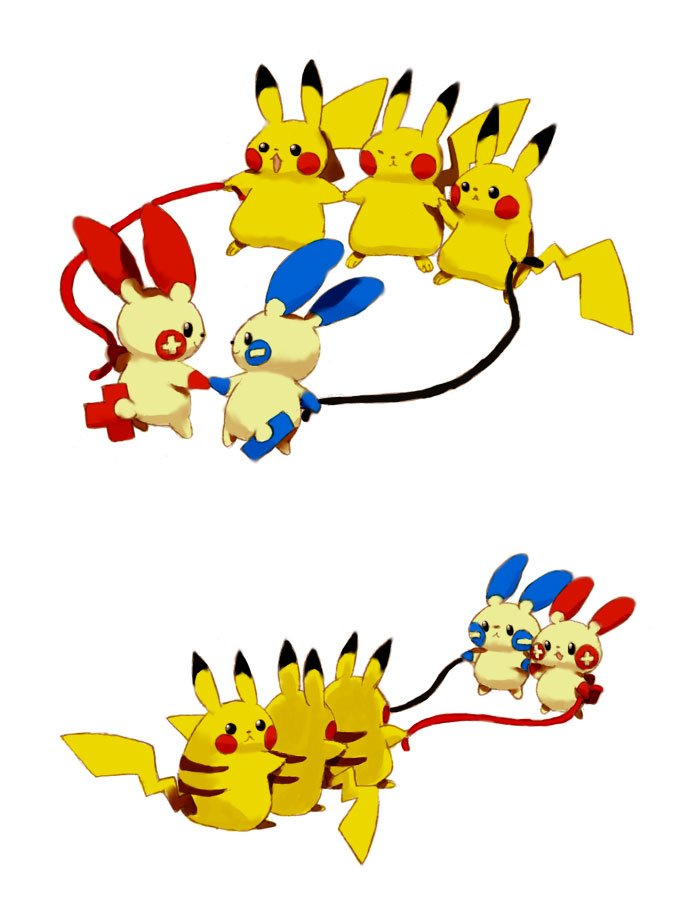
\includegraphics[width=5cm]{07-circuits-cc/figures/series-parallel-pikachu.jpg}
\end{center}
\begin{flushright}
  {\tiny \url{http://i.imgur.com/4fPjx.jpg} }
\end{flushright}

Quelle est la valeur du rapport $\frac{R_s}{R_p}$?

\begin{enumerate}
  \item 9
  \item 3
  \item 1
  \item 1/3
  \item 1/9
\end{enumerate}

\end{diapobox}




\section{Circuits à plusieurs mailles}

\marginnote{
  Tremblay \S 6.8

  Lafrance \S 7.6
}

\minisec{Objectif}
\begin{enumerate}
  \item L'étudiant pourra calculer le courant et la tension dans différent circuits.
\end{enumerate}


\subsection*{Exemple}

\marginpar{Diapo}
Considérons le circuit suivant dans lequel $\emf_1 = \SI{12}{V}$, $\emf_2 =
\SI{9}{V}$, $R_1 = \SI{100}{\ohm}$, $R_2 = \SI{2}{\kilo\ohm}$, $R_3 =
\SI{200}{\ohm}$ et $R_4 = \SI{300}{\ohm}$.
On cherche le courant dans chaque branche du circuit.

\begin{center}
  \begin{circuitikz}
    % French babel breaks everything... see https://latex.org/forum/viewtopic.php?t=11981
    \shorthandoff{:}\shorthandoff{!}
    \draw (0, 0) to[R=$R_1$] (0, 4)
      to[battery, l=$\emf_1$, -*] (4, 4) node[above] {$a$};
    \draw (4, 4) to[R=$R_3$] (8, 4)
      to (8, 0)
      to[R=$R_4$] (4, 0)
      to (0, 0);
    \draw (4, 0) to[battery, l=$\emf_2$] (4, 2)
      to[R=$R_2$] (4, 4);
    \draw[->, black!50!green, thick] (2.5, 0.3) -- node[above] {$i_1$} ++(-1, 0);
    \draw[<-, black!50!green, thick] (4.5, 2.5) -- node[right] {$i_2$} ++(0, -1);
    \draw[->, black!50!green, thick] (5.5, 3.6) -- node[below] {$i_3$} ++(1, 0);
    \draw[black!40!red, thick, ->] (2, 2) node {$1$} ++(230:0.6) arc(230:-50:0.6);
    \draw[black!40!red, thick, ->] (6, 2) node {$2$} ++(230:0.6) arc(230:-50:0.6);
  \end{circuitikz}
\end{center}

\begin{align*}
  \text{Maille 1:} -R_1 i_1 - \emf_1 + R_2 i_2 + \emf_2 &= 0 \\
  \text{Maille 2:} -\emf_2 - R_2 i_2 - R_3 i_3 - R_4 i_3 &= 0 \\
  \text{N\oe ud } a: i_1 + i_2 - i_3 &= 0 \\
\end{align*}

Pour simplifier les calculs, on peut récrire ces équations avec les valeurs
numériques qu'on connaît.
\begin{align}
  \text{Maille 1:} -\SI{100}{\ohm}\cdot i_1 - \SI{12}{V} + \SI{2000}{\ohm}\cdot
    i_2 + \SI{9}{V} &= 0 \nonumber \\
  -\SI{100}{\ohm}\cdot i_1 + \SI{2000}{\ohm}\cdot i_2 - \SI{3}{V} &= 0
  \label{eq:maille1}
  \\[4mm]
  \text{Maille 2:} -\SI{9}{V} - \SI{2000}{\ohm}\cdot i_2 - \SI{200}{\ohm}\cdot i_3 -
    \SI{300}{\ohm}\cdot i_3 &= 0  \nonumber \\
  -\SI{9}{V} - \SI{2000}{\ohm}\cdot i_2 - \SI{500}{\ohm}\cdot i_3 &= 0
  \label{eq:maille2}
  \\[4mm]
  \text{N\oe ud } a: i_1 + i_2 - i_3 &= 0
  \label{eq:noeuda}
\end{align}
De l'équation \ref{eq:maille1}, on a
\[
  i_1 = \frac{\SI{2000}{\ohm}\cdot i_2 - \SI{3}{\volt}}{\SI{100}{\ohm}}
      = 20i_2 - \SI{30}{mA}
\]
De l'équation \ref{eq:maille2}, on a
\[
  i_3 = \frac{-\SI{9}{V} - \SI{2000}{\ohm}\cdot i_2}{\SI{500}{\ohm}}
      = -\SI{18}{mA} - 4i_2
\]
En remplaçant ces deux équations dans l'éqation \ref{eq:noeuda} on obtient
\begin{align*}
  20i_2 - \SI{30}{mA} + i_2 - (-\SI{18}{mA} - 4i_2) &= 0  \\
  25i_2 - \SI{12}{mA} &= 0  \\
  i_2 &= \SI{0.48}{mA}
\end{align*}
D'où on tire que $i_1 = \SI{-20.4}{mA}$ et $i_3 = \SI{-19.92}{mA}$. On conclut
donc que $i_1$ et $i_2$ étaient mal orientés sur le schéma. On a donc des
courants
\begin{align*}
  i_1 &= \SI{20.4}{mA}  \\
  i_2 &= \SI{0.48}{mA}  \\
  i_3 &= \SI{19.92}{mA}
\end{align*}
orientés tel qu'illustré ci-dessous.


\begin{center}
  \begin{circuitikz}[scale=0.9]
    % French babel breaks everything... see https://latex.org/forum/viewtopic.php?t=11981
    \shorthandoff{:}\shorthandoff{!}
    \draw (0, 0) to[R=$R_1$] (0, 4)
      to[battery, l=$\emf_1$, -*] (4, 4) node[above] {$a$};
    \draw (4, 4) to[R=$R_3$] (8, 4)
      to (8, 0)
      to[R=$R_4$] (4, 0)
      to (0, 0);
    \draw (4, 0) to[battery, l=$\emf_2$] (4, 2)
      to[R=$R_2$] (4, 4);
    \draw[<-, black!50!green, thick] (2.5, 0.3) -- node[above] {$i_1$} ++(-1, 0);
    \draw[<-, black!50!green, thick] (4.5, 2.5) -- node[right] {$i_2$} ++(0, -1);
    \draw[<-, black!50!green, thick] (5.5, 3.6) -- node[below] {$i_3$} ++(1, 0);
  \end{circuitikz}
\end{center}


\section{Charge et décharge d'un condensateur}

\minisec{Objectif}

\marginnote{
  Tremblay \S 7.6

  Lafrance \S 7.7
}

\begin{enumerate}
  \item L'étudiant comprendra comment le courant fluctue lorsqu'on charge ou
    qu'on décharge un condensateur.
\end{enumerate}

\subsection*{Démonstration}

On prend deux résistances (\SI{200}{\ohm} et \SI{1000}{\ohm}) et deux
condensateurs (\SI{500}{\micro\farad} et \SI{1000}{\micro\farad}). On montre
que le temps de charge et de décharge est proportionnel à la résistance et à la
capacité.


\subsection*{Raisonnement intuitif}

Capacité plus élevée $\implies$ plus de charges (différence de potentiel
identique au départ) donc courant pendant un plus long moment.

Résistance plus élevée $\implies$ courant plus faible donc plus long pour que
toutes les charges passent.



\subsection{Décharge d'un condensateur}

Appliquer la loi des mailles (conservation de l'énergie) au circuit suivant
pour déterminer le lien entre le courant et le temps.

\begin{center}
\begin{circuitikz}
    % French babel breaks everything... see https://latex.org/forum/viewtopic.php?t=11981
    \shorthandoff{:}\shorthandoff{!}
  \draw (0, 0)
    to[C, l=$C$] (0, 3)
    to (4, 3)
    to[R, l=$R$] (4, 0)
    to (0, 0);
\end{circuitikz}
\end{center}

\begin{align*}
  -RI + \frac{Q}{C} &= 0 \\
  -R \abs{\frac{dQ}{dt}} + \frac{Q}{C} &= 0 \\
  R \frac{dQ}{dt} + \frac{Q}{C} &= 0
\end{align*}

C'est une équation différentielle linéaire du premier ordre. On peut résoudre
par séparation de variables.

\begin{align*}
  \frac{dQ}{dt} &= -\frac{Q}{RC} \\
  \frac{dQ}{Q} &= \frac{-dt}{RC} \\
  \ln\abs{Q} &= \frac{-t}{RC} + k
\end{align*}

On sait que $Q$ est la charge sur la plaque positive donc $\abs{Q} = Q$. À $t =
0$, la charge est la charge initiale $Q_0$. On peut utiliser cette condition
initiale pour trouver la valeur de la constante d'intégration.

\begin{align*}
  \ln Q_0 &= k
\end{align*}

Donc

\begin{align*}
  \ln Q - \ln Q_0 &= \frac{-t}{RC} \\
  \ln \frac{Q}{Q_0} &= \frac{-t}{RC} \\
  \frac{Q}{Q_0} &= e^{-t/RC} \\
  Q(t) &= Q_0 e^{-t/RC}
\end{align*}


\marginnote{
  \begin{center}
  \begin{tikzpicture}[xscale=0.8, yscale=1.2]
    \draw plot[domain=0:4] (\x, {exp(-\x)});
    \draw (0, 0) -- (0, 1.4) node[left] {$Q$};
    \draw (0, 0) -- (4.5, 0) node[below] {$t$};
    \draw (0, 1) -- ++(-0.1, 0) node[left] {$Q_0$};
  \end{tikzpicture}
  \end{center}
}

Au départ, la charge décroit rapidement car la différence de potentiel est
élevée donc les charges veulent aller vers l'autre plaque. Plus la différence
de potentiel diminue, moins les charges sont \og motivées \fg\ à aller vers
l'autre plaque donc la charge diminue de moins en moins rapidement.

Quelle est la limite de validité de ce modèle?

Si la charge est trop petite, on se heurte à la quantification de la charge.
Notre modèle est correct tant que la charge est assez grande pour qu'on puisse
la considérer comme continue.



\minisec{Demi-vie et constante de temps}

Combien de temps faut-il pour décharger le condensateur jusqu'à ce que sa
charge soit la moitiée de la charge initiale?

\begin{align*}
  Q(t_{1/2}) = \frac{Q_0}{2} &= Q_0 e^{-t_{1/2} / RC} \\
  \frac{1}{2} &= e^{-t_{1/2} / RC} \\
  \frac{-t_{1/2}}{RC} &= \ln 2 \\
  t_{1/2} = RC \ln 2
\end{align*}

C'est le temps de demi-vie.

Quelles sont les unités de $RC$?

$\tau = RC$ est la constante de temps pour le circuit $RC$. De combien a
diminué la charge lorsque $t = RC$?


\subsection{Charge d'un condensateur}

Essayez de déterminer l'expression pour la charge en fonction du temps sur un
condensateur qu'on charge.

\begin{center}
\begin{circuitikz}
    % French babel breaks everything... see https://latex.org/forum/viewtopic.php?t=11981
    \shorthandoff{:}\shorthandoff{!}
  \draw (0, 0)
    to[C, l=$C$] (0, 3)
    to[battery, l=\emf] (4, 3)
    to[R, l=$R$] (4, 0)
    to (0, 0);
\end{circuitikz}
\end{center}

On applique la loi des mailles
\begin{align*}
  \emf - RI - \frac{Q}{C} &= 0 \\
  \emf - R \abs{\frac{dQ}{dt}} - \frac{Q}{C} &= 0 \\
  \emf - R \frac{dQ}{dt} - \frac{Q}{C} &= 0 \\
  \frac{dQ}{dt} &= \frac{C\emf - Q}{RC} \\
  \frac{dQ}{C\emf - Q} &=  \frac{dt}{RC} \\
  -\ln \abs{C\emf - Q} &= \frac{t}{RC} + k \\
  \ln \abs{C\emf - Q} &= \frac{-t}{RC} - k \\
\end{align*}

$C\emf$ est la charge maximale que le condensateur peut supporter, $Q_m$.
\begin{align*}
  \ln (Q_m - Q) &= \frac{-t}{RC} - k
\end{align*}

À $t = 0$, $Q = 0$, donc
\begin{align*}
  \ln Q_m &= -k \\
  \ln \frac{Q_m - Q}{Q_m} &= \frac{-t}{RC} \\
  1 - \frac{Q}{Q_m} &= e^{-t/RC} \\
  Q &= Q_m \left( 1 - e^{-t/RC} \right)
\end{align*}


\begin{diapobox}
  \minisec{Défibrillateur}
  Un défibrillateur cardiaque est composé d'une source de tension dont la fém est
  \SI{2500}{V} et d'un condensateur de \SI{32}{\micro\farad}. Pour charger le
  condensateur, on le place en série avec une résistance de \SI{10}{\kilo\ohm}.

  Quel est le temps requis pour que le condensateur atteigne \SI{95}{\percent} de
  sa charge maximale?
\end{diapobox}

\begin{reponsebox}
\begin{align*}
  \Delta V &= \emf \left( 1 - e^{-t/RC} \right)  \\
  e^{-t/RC} &= 1 - \frac{\Delta V}{\emf}  \\
  \frac{-t}{RC} &= \ln\left( 1 - \frac{\Delta V}{\emf} \right)  \\
  t &= -RC \ln\left( 1 - \frac{\Delta V}{\emf} \right)  \\
    &= -RC \ln\left( 1 - \num{0.95} \right)  \\
    &= \SI{0.9586}{s}
\end{align*}
\end{reponsebox}

\begin{diapobox}
  Maintenant que le condensateur est chargé, on peut utiliser le défibrillateur.
  On connecte le condensateur en série avec le c\oe ur et le condensateur se
  décharge à travers ce dernier. La décharge dans le c\oe ur prend \SI{5}{ms} et
  est complète lorsqu'il ne reste que \SI{10}{\percent} des charges initiales
  sur le condensateur. Quelle est la résistance du thorax?

  Quel était le courant dans le c\oe ur \SI{1}{ms} après le
  début de la décharge?

  Quelle est l'énergie qui est fournie par le condensateur au c\oe ur?
\end{diapobox}

\begin{reponsebox}
  \begin{align*}
    \Delta V &= \Delta V_0 e^{-t/R_tC}  \\
    e^{-t/R_tC} &= \frac{\Delta V}{\Delta V_0}  \\
    \frac{-t}{R_tC} &= \ln\left( \frac{\Delta V}{\Delta V_0} \right)  \\
    R_t &= -\frac{t}{C\ln\left( \num{0.1} \right)}  \\
        &= \SI{67.86}{\ohm}
  \end{align*}

  \begin{align*}
    I &= I_0 e^{-t/R_tC}  \\
      &= \frac{\Delta V_0}{R_t} e^{-t/R_tC}  \\
      &= \SI{22.08}{A}
  \end{align*}

  \begin{align*}
    U &= \frac{1}{2} C (\Delta V_0^2 - \num{0.1} \Delta V_0^2)  \\
      &= \SI{81.23}{J}
  \end{align*}
\end{reponsebox}
